\section{Three-tier architecture}

The three-tier architecture comprises a server for data management, a client for presentation layout, and a middle tier to enhance the separation between the client and the server.
\begin{figure}[H]
    \centering
    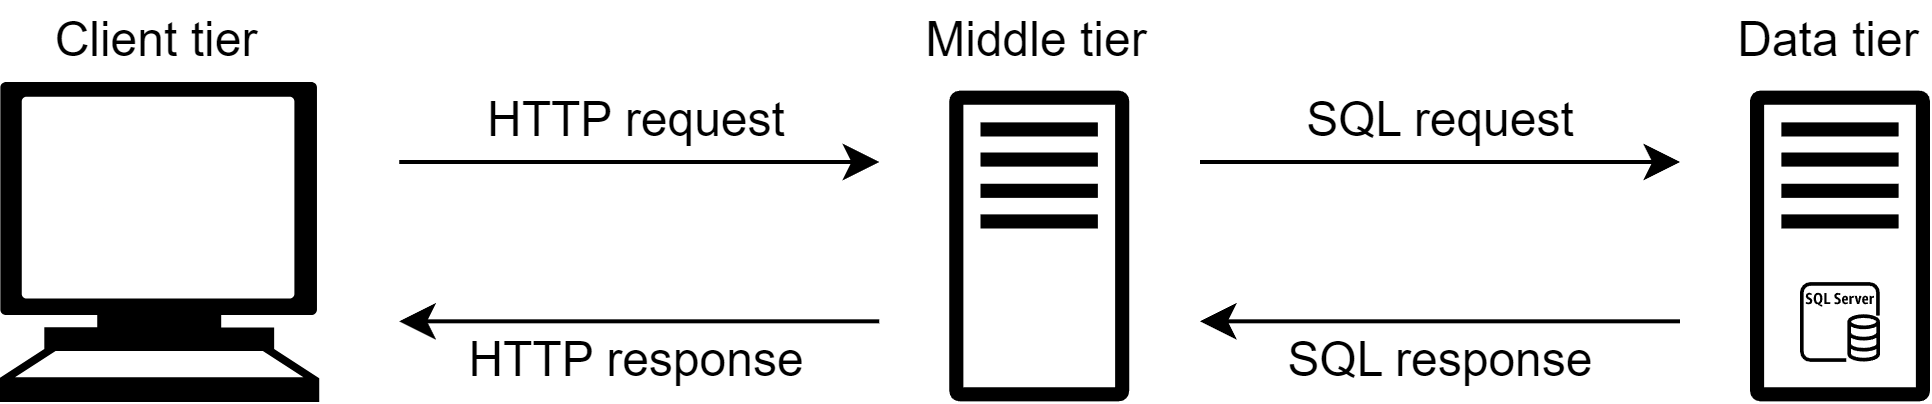
\includegraphics[width=0.5\linewidth]{images/ttph.png}
\end{figure}
This architecture has several variants, depending on the software features of the middle tier:
\begin{itemize}
    \item \textit{Web Pure HTML}: the client functions as a standard web browser, focusing solely on the presentation layout (thin client). 
        The middle tier incorporates a web server utilizing HTTP, hosts the business logic for dynamically generating content from the raw data of the data tier, and manages the presentation layout.
    \item \textit{Rich Internet Application} (RIA): his is a fusion of web and desktop applications using JavaScript.
        The client is termed fat due to its standard communication protocol, language, and API. 
        Noteworthy features of this architecture include novel interface event types, including those specific to touch and mobile apps, asynchronous interaction (AJAX), client-side persistent data, offline application capabilities, and native multimedia and 3D support.
\end{itemize}